\documentclass{beamer}
\usecolortheme{whale}
\usepackage[utf8]{inputenc}
\usepackage{dirtytalk,amsmath,tikz,mathtools,amsmath}
\usepackage{resizegather}
\usetikzlibrary{automata, positioning}
\graphicspath{ {./images/} }
\tikzset{->, initial text=$$}
\DeclareMathAlphabet{\mathpzc}{OT1}{pzc}{m}{it}
%Information to be included in the title page:
\title{Logic and Hybrid Systems}
\author{Manasvi Saxena}
\institute{Formal Systems Lab, UIUC}
\date{}

\setbeameroption{hide notes} % Only slides
%\setbeameroption{show only notes} % Only notes
%\setbeameroption{show notes on second screen=right} % Both
\setbeamertemplate{note page}{\pagecolor{yellow!5}\insertnote}\usepackage{palatino}
\setbeamerfont{caption}{size=\scriptsize}

\newcommand{\dL}{\text{\upshape\textsf{d{\kern-0.05em}L}}}
\newcommand{\Trm}{\text{Trm}}
\newcommand{\HP}{\text{HP}}
\newcommand{\accel}{\textit{accel}}
\newcommand{\brake}{\textit{brake}}
\newcommand{\R}{\mathbb{R}}
\newcommand{\val}[4]{\textit{val}_{#1, #2}(#3, #4)}
\newcommand{\valDefault}[1]{\val{I}{\eta}{\nu}{#1}}
\newcommand{\transRel}[3]{\rho_{#1, #2}(#3)}
\newcommand{\transRelDef}[1]{\transRel{I}{\eta}{#1}}
\newcommand{\z}{\mathpzc{Z}}

\begin{document}

\frame{\titlepage}

\begin{frame}
\frametitle{Hybrid Systems}

\begin{itemize}
  \item Dynamical Systems exhibiting both discrete (jump) and continuous (flow) behaviors.
  \item Physical systems - thermostats, airplanes and trains.
  \item Continuous dynamics generally specified using Differential Equations.
\end{itemize}

\end{frame}

\begin{frame}
  \frametitle{Differential Dynamic Logic (\dL)}
  \begin{itemize}
    \item Main focus - Differential Dynamic Logic for Hybrid Systems (Andre
      Platzer).
      \pause
    \item Practical deductive verification of hybrid systems.
    \item Introduces Hybrid Program - program notation for hybrid systems.
    \item Dynamic Logic for Hybrid Programs, a generalization of Dynamic Logic.
  \end{itemize}

\end{frame}

\begin{frame}
\frametitle{Hybrid Automata}
\begin{itemize}
  \item Commonly used to model Hybrid Systems, via Graphs.
  \item Nodes specify continuous dynamics. Edges describe discrete transitions.
  \item Intuitive, but not suitable for deductive verification.
\end{itemize}
    \pause
\begin{figure}\label{fig:train-HA}
  \centering
  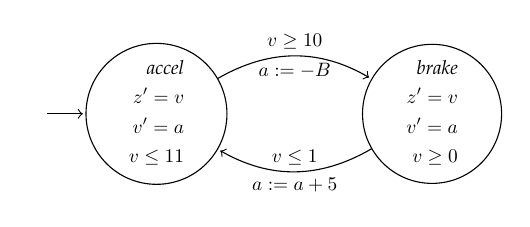
\begin{tikzpicture}[shorten >=1pt,node distance=5cm,on grid,auto]
    
  \node[state,initial, scale=0.70] (accel)   {%
  $\begin{aligned}
      \textit{accel} \\
      z' = v \\
      v' = a \\
      v \leq 11
  \end{aligned}$
  };

  \node[state,scale=0.70] (brake) [right of = accel] {%
  $\begin{aligned}
      \textit{brake} \\
      z' = v \\
      v' = a \\
      v \geq 0
  \end{aligned}$
   };

   \draw (accel) edge[bend left, above] node[midway,below,scale=0.7] {$a := -B$}
   node[midway,above,scale=0.7] {$v \geq 10$} (brake);
   \draw (brake) edge[bend left, below] node[midway,below,scale=0.7] {$a := a+5$}
   node[midway,above,scale=0.7] {$v \leq 1$} (accel);

  \end{tikzpicture}
  \caption{Hybrid Automata (simplified) of a Train Control System}
\end{figure}
\end{frame}

\begin{frame}{Differential Dynamic Logic}{Motivations}
  \begin{itemize}
    \item \textbf{First Order Logic} - No builtin means for referring to state
      transitions.
    \item \textbf{Temporal Logics} - Modal operators allow referring to state transitions.
      But valid formulas only express generic facts.
      \end{itemize}
\end{frame}
\begin{frame}
    \textbf{Dynamic Logic (DL)} - Combines operational system models with
      operators for reasoning.
      \begin{itemize}
        \item Provides parameterized modal operators, $[\alpha]$,
          $\langle\alpha\rangle$
          that refer to states reachable by system $\alpha$.
        \item $[\alpha]\phi$ expresses all states reachable by $\alpha$ satisfy
          $\phi$, allowing reasoning about discrete systems.
        \item Say $(b > 0) \to [a := -b] (a < 0) $ expresses a
          discrete transition. We can prove $(b > 0) \vdash (a < 0) [ b / a ]$
          using DL's calculus.
        \item No built in notion for describing or reasoning about continuous dynamics.
      \end{itemize}
\end{frame}

\begin{frame}{Differential Dynamic Logic}{Motivations}
  \begin{itemize}
    \item Generalize DL so operational models $\alpha$ can be
      used in modal formulas like $[\alpha]\phi$. $\dL$ refers to
      generalized models as \say{Hybrid Programs}.
  \end{itemize}
\end{frame}

\begin{frame}{Differential Dynamic Logic}{Syntax and Semantics}
    $\dL$ formulas built over
    \begin{itemize}
      \item $V$, set of real-valued logical variables.
      \item Signature $\Sigma = \Sigma_{\text{rigid}} \cup \Sigma_{\text{fl}}$
      \item Set $\text{Trm}(\Sigma,V)$ of \textit{terms} - classical FOL polynomial
        expressions over $V$ with additional skolem terms $s(X_1, \dots,
   X_n)$, where $X_1, \dots, X_n \in V$.
 \end{itemize}
\end{frame}

\begin{frame}{Differential Dynamic Logic}{Syntax and Semantics}
  \begin{block}{Hybrid Programs}
  Consider $x_i \in \Sigma$, $\theta_i, \vartheta_i \in \Trm(\Sigma, V)$ for
  $1 \leq i \leq n$, $\chi$ a $(\Sigma,V)$ FOL-formula, $\alpha, \beta \in
  \HP(\Sigma,V)$.
    Set $\HP(\Sigma,V)$, is defined inductively as -
    \begin{itemize}
      \item  $(x_1 := \theta_1, \ldots , x_n := \theta_n) \in \HP(\Sigma,V)$
      \item $ (x'_1 = \vartheta_i, \ldots , x'_n = \vartheta_n)\, \& \, \chi \in
        \HP(\Sigma,V)$. $x'_i = \vartheta_i$ is a differential equation where
        $x'_i$ is the first order time derivative of $x_i$.
      \item $(?\chi) \in \HP(\Sigma,V)$.
      \item $\alpha \cup \beta \in \HP(\Sigma, V)$.
      \item $\alpha;\beta \in \HP(\Sigma, V)$.
      \item $\alpha^* \in \HP(\Sigma, V)$.
    \end{itemize}
  \end{block}
\end{frame}


\begin{frame}{Differential Dynamic Logic}{Hybrid Program Example}
    \begin{columns}
    \uncover<1,2>{%
    \column{.4\textwidth}
      \begin{figure}
      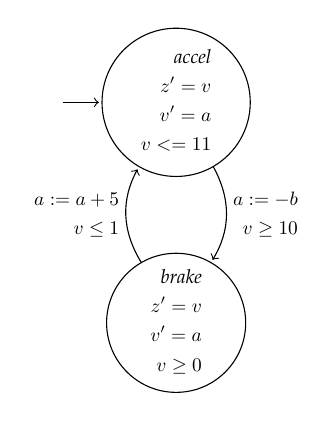
\begin{tikzpicture}[shorten >=1pt,node distance=4cm,on grid,auto]
        
  \node[state,initial, scale=0.70] (accel)   {%
  $\begin{aligned}
      \textit{accel} \\
      z' = v \\
      v' = a \\
      v <= 11
  \end{aligned}$
  };

  \node[state,scale=0.70] (brake) [below of = accel] {%
  $\begin{aligned}
      \textit{brake} \\
      z' = v \\
      v' = a \\
      v \geq 0
  \end{aligned}$
   };

   \draw (accel) edge[bend left, left] node[right,scale=0.7](t1) {%
     $\begin{aligned}
       a := -b \\
       v \geq 10
     \end{aligned}$
   } (brake) ;
   \draw (brake) edge[bend left, right] node[left,scale=0.7](t2) {%
     $\begin{aligned}
       a := a + 5 \\
       v \leq 1
     \end{aligned}$
   }(accel);

      \end{tikzpicture}
      \caption{Hybrid Automata of Simple Train Control System}
      \end{figure}
    }
    \uncover<2>{%
    \column{.6\textwidth}
    \begin{equation*}
    \begin{split}
      & q := \accel ; \\
      & ( (?q = \accel ; z' = v, v' = a \& v \leq 11) \\
      &  \cup (?q = \accel \wedge v \geq 10 ; a := - b; q:=\brake ; ?v \geq 0) \\
      &  \cup (?q = \brake; z' = v,v' =a \& v \geq 0) \\
      &  \cup (?q = \brake \wedge \leq 1; a := a + 5; q:=\accel) )*
      \end{split}
    \end{equation*}
  }
    \end{columns}
\end{frame}
\begin{frame}{Differential Dynamic Logic}{Syntax and Semantics}
  \begin{block}{$\dL$ Formulas}
    The set $\text{Fml}(\Sigma,V)$ of $\dL$ formulas is defined as -
    \begin{itemize}
      \item If $p$ is a n-ary predicate symbol in $\Sigma$ and $\theta_1,
        \ldots, \theta_n \in \text{Trm}(\Sigma,V)$, then $p(\theta_1, \ldots,
        \theta_n) \in \text{Fml}(\Sigma,V)$
      \item If $\phi, \psi \in \text{Fml}(\Sigma,V)$ then $\phi \vee \psi, \phi
        \to \psi, \phi \wedge \psi \in \text{Fml}(\Sigma,V)$
      \item If $\phi \in \text{Fml}(\Sigma,V)$ and $x \in V$  then
        $\exists x . \phi, \forall x.\phi \in \text{Fml}(\Sigma,V)$
      \item If $\phi \in \text{Fml}(\Sigma,V)$ and $\alpha \in
        \text{HP}(\Sigma,V)$  then
        $ [\alpha]\phi, \langle \alpha \rangle\phi \in \text{Fml}(\Sigma,V)$
    \end{itemize}
  \end{block}
\end{frame}

\begin{frame}{Differential Dynamic Logic}{Syntax and Semantics}
  \begin{block}{Some Notation}
    \begin{itemize}
      \item Interpretation $I: \Sigma_text{rigid} \to \mathbb{R}$
      \item A state is a map $\nu : \Sigma_{\textit{fl}} \to \R$.
      \item Assignment of logical variables is a map $\eta : V \to \R$.
      \item The models are Kripke Structures, where nodes are
        hybrid system states.
    \end{itemize}
  \end{block}
\end{frame}

\begin{frame}{Differential Dynamic Logic}{Syntax and Semantics}
    \begin{block}{$\dL$ Valuation of $\dL$ Terms}
      Say $\valDefault{\cdot}$ is evaluation w.r.t. interpretation $I$, assignment $\eta$ and state $\nu$.
      \pause
      \begin{itemize}
      \item (State Variables) $\valDefault{a} = \nu(a), x \in \Sigma_{\textit{fl}}$
        \pause
      \item (Logical Variables) $\valDefault{x} = \eta(x), x \in V$
        \pause
      \item (Rigid Symbols) $\valDefault{f(\theta_1, \ldots, \theta_n)} =
          f_I(\valDefault{\theta_1}, \ldots, \valDefault{\theta_n})$ \\
          where $f$ is n-ary rigid symbol in $\Sigma$
      \end{itemize}
    \end{block}
\end{frame}

\begin{frame}{Differential Dynamic Logic}{Syntax and Semantics}
    \begin{block}{Valuation of $\dL$ Formulas}
      \begin{itemize}
      \item $\valDefault{p(\theta_1, \ldots, \theta_n)} = p_I(\valDefault{\theta_1}, \ldots, \valDefault{\theta_n})$
      \item $\valDefault{\varphi \wedge \psi} = \top$ iff
        $\valDefault{\varphi} = \top \wedge \valDefault{\psi} = \top$.
        Similarly for $\to, \neg, \vee$
      \item $\valDefault{\exists x \ldotp \varphi} = \top$ iff
        $\val{I}{\eta[x \mapsto d]}{\nu}{\varphi} = \top$ for some $d \in \R$
      \pause
      \item $\valDefault{[\alpha]\varphi} = \top$ iff
        $\val{I}{\eta}{\omega}{\varphi} = \top$ for all states $\omega$ with $(\nu, \omega)
        \in \transRelDef{\alpha}$.
      \item $\valDefault{\langle\alpha\rangle\varphi} = \top$ iff
        $\val{I}{\eta}{\omega}{\varphi} = \top$ for some state $\omega$ with $(\nu, \omega)
        \in \transRelDef{\alpha}$.
      \end{itemize}
    \end{block}
\end{frame}

\begin{frame}{Differential Dynamic Logic}{Syntax and Semantics}
  \begin{block}{Transition Semantics of Hybrid Programs}
    Evaluation $\transRelDef{\alpha}$ of HP $\alpha$. $(\nu, \omega) \in
    \transRelDef{\alpha}$ means state $\omega$ is reachable from $\nu$ by
    operations of $\alpha$.
    \begin{itemize}
      \item $(\nu, \omega) \in \transRelDef{x_1 := \theta_1, \dots, x_n := \theta_n}$
        iff $\nu[x_1 \mapsto \valDefault{\theta_1}, \ldots, x_n \mapsto
        \valDefault{\theta_n}]
       = \omega$ and $\forall y \in (\Sigma_{\textit{fl}} - \{x_1, \ldots,
       x_n\}). \val{I}{\eta}{\nu}{y} = \val{I}{\eta}{\omega}{y}$.
       \pause
     \item $\transRelDef{\alpha \cup \beta} = \transRelDef{\alpha} \cup
       \transRelDef{\beta}$
       \pause
     \item $\transRelDef{?\chi} = \{(\nu,\nu) : \valDefault{\chi} = \top \}$
       \pause
     \item $\transRelDef{\alpha ; \beta} = \{(\nu,\omega) : (\nu, \mathpzc{Z}) \in
         \transRelDef{\alpha} \wedge (\mathpzc{Z},\omega) \in \transRelDef{\beta}
       \text{ for some state } \mathpzc{Z}\}$
       \pause
     \item $ (\nu, \omega) \in \transRelDef{\alpha^*}$ iff for $n \in
       \mathbb{N}$, there are states $\nu = \nu_0,\ldots,\nu_n = \omega$ s.t.
       $(\nu_i, \nu_{i+1}) \in \transRelDef{\alpha}$ for $0 \leq i < n$.
    \end{itemize}
  \end{block}
\end{frame}

\begin{frame}{Differential Dynamic Logic}{Syntax and Semantics}
  \begin{block}{Transition Semantics of Hybrid Programs}
      $(\nu, \omega) \in \transRelDef{(x_1' = \vartheta_1 \ldots x_n' =
        \vartheta_n) \& \chi}$ iff there is a flow of some duration $r \geq 0$,
        from $\nu$ to $\omega$ respecting the differential equations and evolution
        domain. Formally, there is a function $f : [0,r] \to \text{Sta}(\Sigma)$ such that -
        \begin{itemize}
          \item $f(0) = \nu$ and $f(r) = \omega$.
          \item $\forall \delta : [0,r] . \val{I}{\eta}{f(\delta)}{x_i}$ is
            continuous and $\val{I}{\eta}{f(\delta)}{\chi} = \top$.
          \item  $\forall \epsilon : (0,r) .
            \val{I}{\eta}{f(\epsilon)}{\vartheta_i} = \dot{f}(\epsilon)$.
          \item For any $ z \not \in \{x_1, x_2, \ldots, x_n\} $,
            $\val{I}{\eta}{f(\zeta)}{z}$ remains constant for $\zeta \in [0,r]$.
            In other words, all other state variables remain unchanged.
        \end{itemize}
  \end{block}
\end{frame}
\begin{frame}{Differential Dynamic Logic}{Syntax and Semantics}
  \begin{columns}[c]
    \column{.5\textwidth}
      \begin{figure}
        \centering
        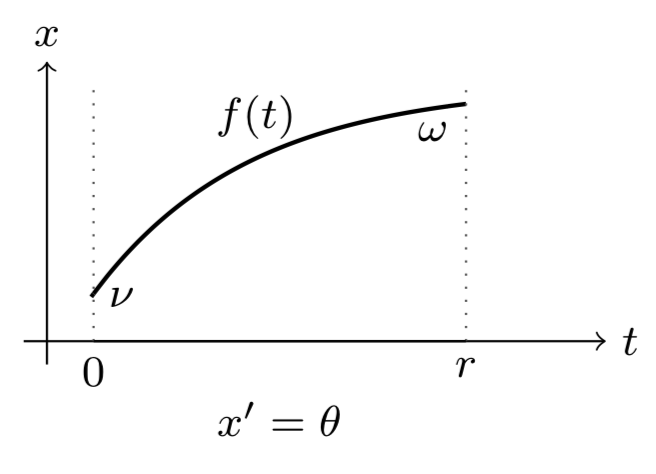
\includegraphics[scale=0.47]{unbounded-evolution}
      \caption{Unbounded Evolution}
      \end{figure}
    \column{.5\textwidth}
      \begin{figure}
        \centering
        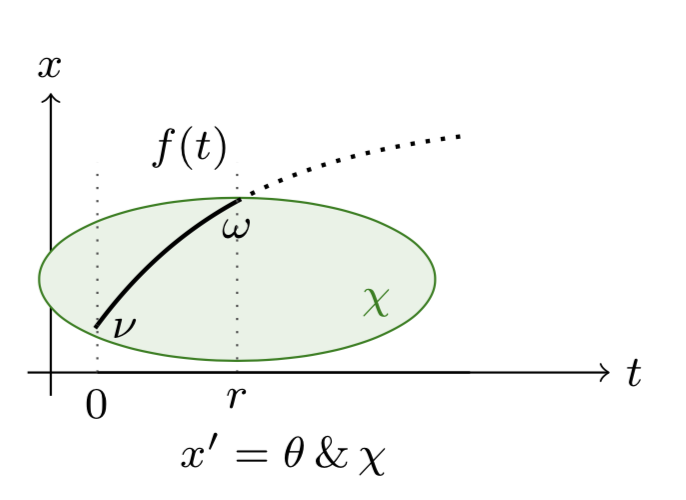
\includegraphics[scale=0.45]{bounded-evolution}
      \caption{Evolution bound by $\chi$}
    \end{figure}
    \end{columns}
\end{frame}

\begin{frame}{Differential Dynamic Logic}{Examples}
  \begin{block}{Some Intuition behind $\dL$}
  \begin{itemize}
    \item Generally, want to reason about Embedded Systems (ES) or Cyber Physical Systems (CPS).
      \pause
    \item Loosely speaking, an ES or CPS is built upon the integration of Computation (Controller) and
      Physical Systems (Plant). Examples include autopilot, ABS (Anti Lock
      Braking Systems), fly-by-wire (human interaction).
    \item Expressed in $\dL$ as an HP $\alpha \equiv (ctrl ; plant)^*$.
      \pause
    \item Formulas of interest are of the form $\varphi \to [\alpha]\psi$.
    \item Formula above says that all states satisfying $\varphi$ will
      always transition to states satisfying $\psi$, where $\alpha$ dictates
      the transition relation.
  \end{itemize}
\end{block}
\end{frame}

\begin{frame}{Differential Dynamic Logic}{Motivating Example}
  \begin{block}{European Train Control System (ETCS)}
    \begin{figure}
      \centering
      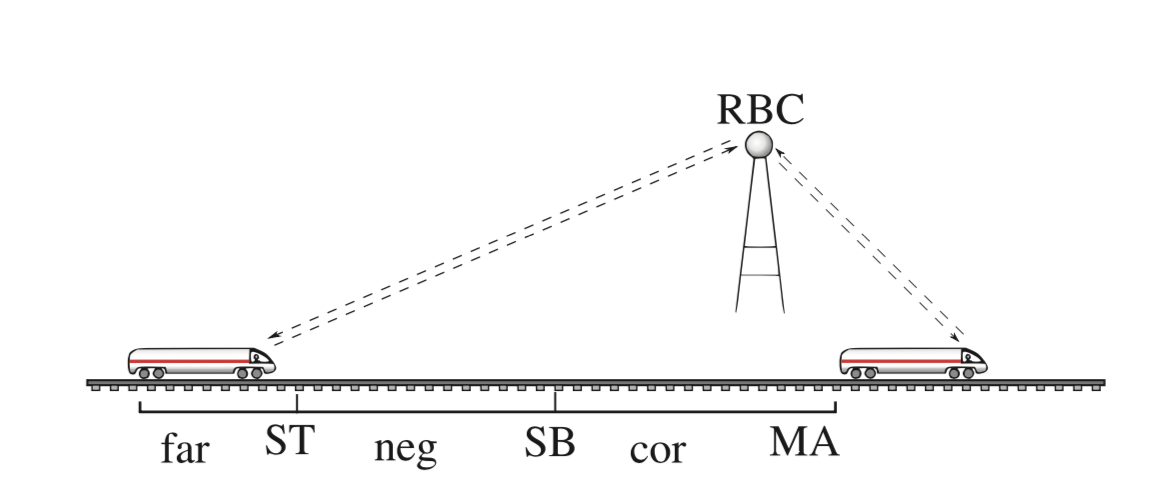
\includegraphics[scale=0.3]{etcs}
    \end{figure}
  \begin{itemize}
    \item <only@1> Discards traditional fixed segments of track with mutual
      exclusion. Instead uses decentralized Radio Block Controllers (RBCs)
    \item <only@1> Trains dynamically issues Movement Authorization (MAs).
    \item <only@1> At the end of MA, agent requests MA extension (negotation).
      If request is denied, train breaks before exiting old MA
      zone.
     \item <only@2> Train controller is responsible for staying in MA.
     \item <only@2> Controller has to determine point SB (Start Braking). Before SB,
      train can move freely (maximizing throughput).
    \item <only@2> Beyond SB (correction phase) start braking such that
      train remains in MA if RBC refuses extension.
  \end{itemize}
  \end{block}
  \end{frame}

\begin{frame}{Differential Dynamic Logic}{Motivating Example}
  \begin{block}{European Train Control System (ETCS)}
    Say we have a train -
    \begin{itemize}
      \item with MA granted upto some track position $m$
      \item at position $\z$, heading with initial speed $v$ towards $m$
      \item point SB as safety distance $s$ relative to $m$, i.e. $m-s = SB$
    \end{itemize}
    \pause
    The following formula expresses that the train remains in its MA under precondition $\psi$.
    \begin{figure}
      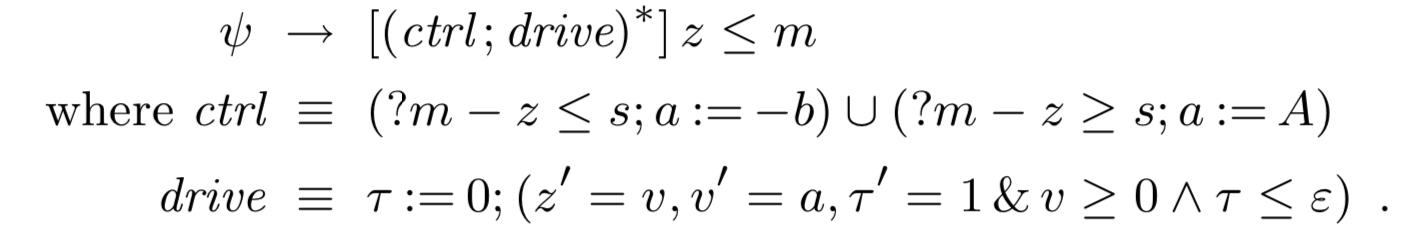
\includegraphics[scale=0.4]{ects-safety}
    \end{figure}
  \end{block}
  \end{frame}

\begin{frame}{Differential Dynamic Logic}{Motivating Example}
  \begin{block}{European Train Control System (ETCS)}
    Say we have a train -
    \begin{itemize}
      \item with MA granted upto some track position $m$
      \item at position $\z$, heading with initial speed $v$ towards $m$
      \item point SB as safety distance $s$ relative to $m$, i.e. $m-s = SB$
    \end{itemize}
    \pause
    The following formula expresses that the train remains in its MA under precondition $\psi$.
    \begin{figure}
      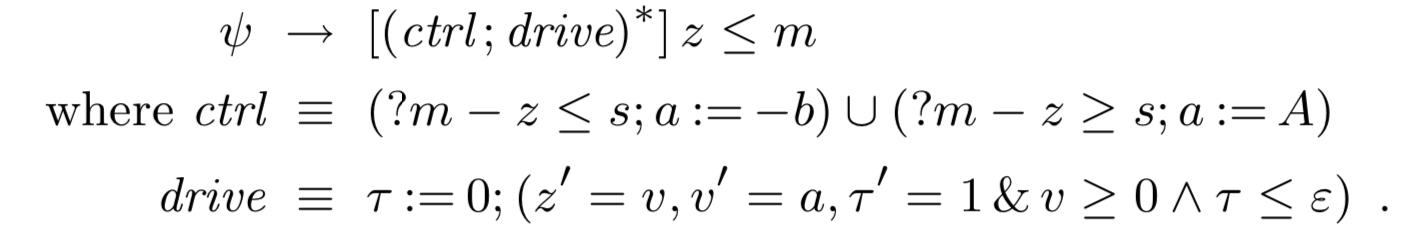
\includegraphics[scale=0.4]{ects-safety}
    \end{figure}
  \end{block}
  \end{frame}

\begin{frame}{Differential Dynamic Logic}{Motivating Example}
  \begin{block}{European Train Control System (ETCS)}
    \begin{figure}
      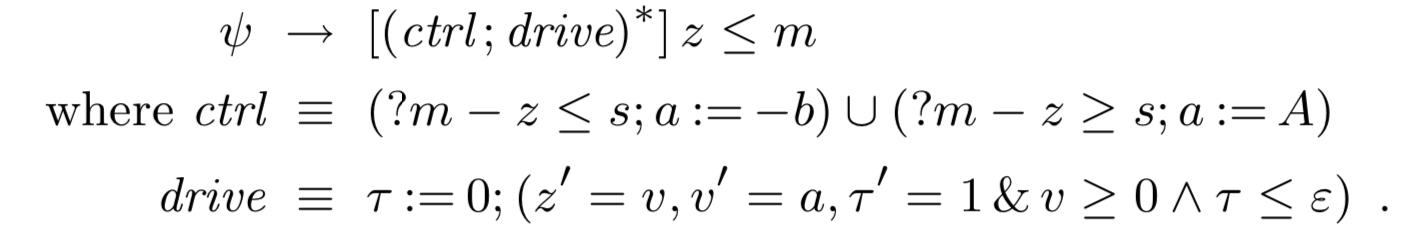
\includegraphics[scale=0.4]{ects-safety}
    \end{figure}
  \end{block}
  \begin{block}{ECTS Safety Verification}
    In order to verify safety, we need
    \begin{enumerate}
      \item Use the calculus to analyze conditions of safety violation. Will
        provide some intuition about the safety precondition.
      \item Use the calculus to verify safety, allowing exploration of the
        calculus' rules.
      \end{enumerate}
  \end{block}
\end{frame}

\begin{frame}{Differential Dynamic Logic}{Proof Calculus}
  \begin{block}{Preliminaries}
    \begin{itemize}
      \item $\phi_{x_1}^{\theta_1}, \ldots, \phi_{x_n}^{\theta_n}$ denotes
        simultaneous substitution of $x_i$ for $\theta_i$ in $\phi$.
      \item Substitution must be \say{admissible}. Given term $t$ and
        substitution $\sigma$, variables of $t$ or $\sigma(t)$ must not occur in
        the scope of a quantifier or modality binding. $\alpha$ conversion for
        renaming is assumed and used when needed.
      \item $\forall^{\alpha}\phi$ denotes the universal closure of $\phi$
        w.r.t. all state variables bound by $\alpha$. Note
        quantification over state variables is definable
        via auxiliary logical variables as $\forall X [x := X] \phi$
      \item The calculus consists of propositional (P), first order (F),
        global (G), dynamic modality (D) rules.
      \item The calculus has 32 rules.
    \end{itemize}
  \end{block}
\end{frame}
\begin{frame}{Differential Dynamic Logic}{Proof Calculus}
  \begin{block}{Discrete Dynamics}
  \begin{figure}
    \centering
    \includegraphics[scale=0.5]{D-discrete-rule}
  \end{figure}
\end{block}
  \begin{block}{Continuous Dynamics}
  \begin{figure}
    \centering
    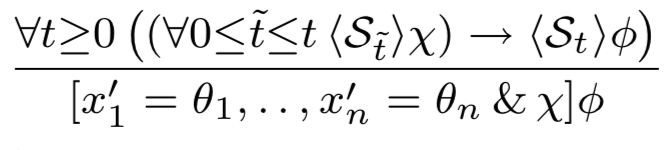
\includegraphics[scale=0.5]{D-continuous-rule}
  \end{figure}
  \begin{itemize}
    \item $t$ and $\tilde{t}$ are fresh logical variables. $\langle S_t \rangle$ is the jump set
      $\langle x_1 := y_1(t), \dots x_n := y_n(t) \rangle$, with simultaneous
      solutions $y_1, \ldots, y_n$ of the respective differential equations with
      constant symbols $x_i$ as symbolic initial values.
  \end{itemize}
\end{block}
\end{frame}

\begin{frame}{Differential Dynamic Logic}{Proof Calculus}
  \begin{block}{F Rules}
  \begin{figure}
    \centering
    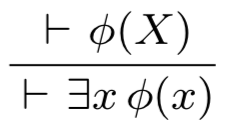
\includegraphics[scale=0.5]{F-existential-rule}
  \end{figure}
  $X$ is a new logical variable.
  \begin{figure}
    \centering
    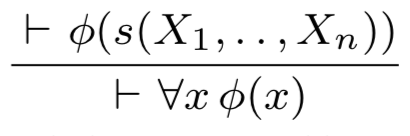
\includegraphics[scale=0.5]{F-universal-rule}
  \end{figure}
  $X_1, \ldots, X_n$ are all free logical variables of $\forall x \phi(x)$
  \end{block}
  F rules are inspired from Tableuax methods for FOL, introducing decision
  procedures into the proof system itself.
\end{frame}


\begin{frame}{Differential Dynamic Logic}{Proof Calculus}
  \begin{block}{F Rules}
  \begin{figure}
    \centering
    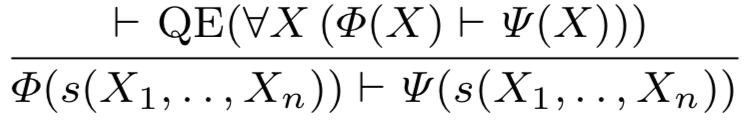
\includegraphics[scale=0.5]{F-reintroduce-forall-rule}
  \end{figure}
    $X$ is a new logical variable
  \begin{figure}
    \centering
    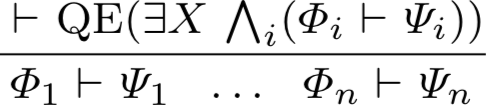
\includegraphics[scale=0.5]{F-introduce-existential-rule}
  \end{figure}
  Logical variable $X$ only occurs in $\Phi_i \vdash \Psi_i$. The intuition
  is variable $X$ was introduced via skolemization (at some point in the proof
  tree). The rule reintroduces existentiality over $X$, allowing for Quantifier
  Elimination (QE) over the existentially quantified terms.
  \end{block}
\end{frame}

\begin{frame}{Differential Dynamic Logic}{Proof Calculus}
  \begin{block}{G Rules}
  \begin{figure}
    \centering
    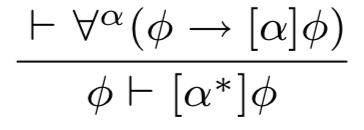
\includegraphics[scale=0.5]{G-introduce-precondition}
  \end{figure}
  \begin{figure}
    \centering
    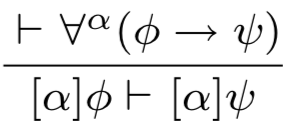
\includegraphics[scale=0.5]{G-model-precondition}
  \end{figure}
  \end{block}
\end{frame}

\begin{frame}{Differential Dynamic Logic}{Proof Calculus Application}
 \begin{block}{European Train Control System (ETCS)}
   \begin{figure}
     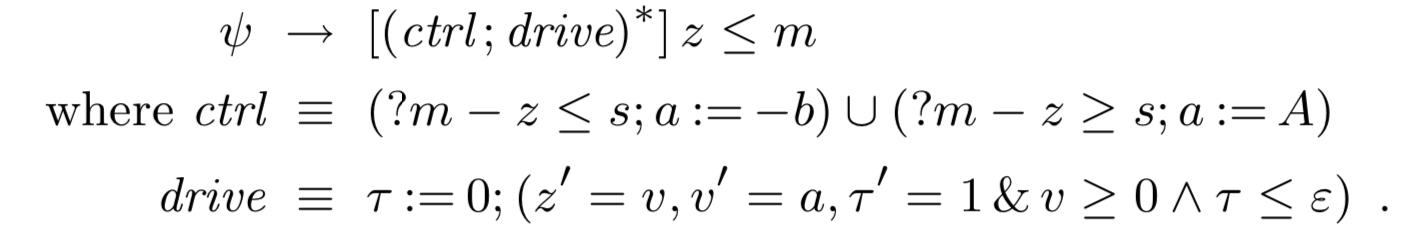
\includegraphics[scale=0.4]{ects-safety}
   \end{figure}
 \end{block}
 \begin{block}{Deduction modulo for MA violation in braking mode}
   \begin{figure}
     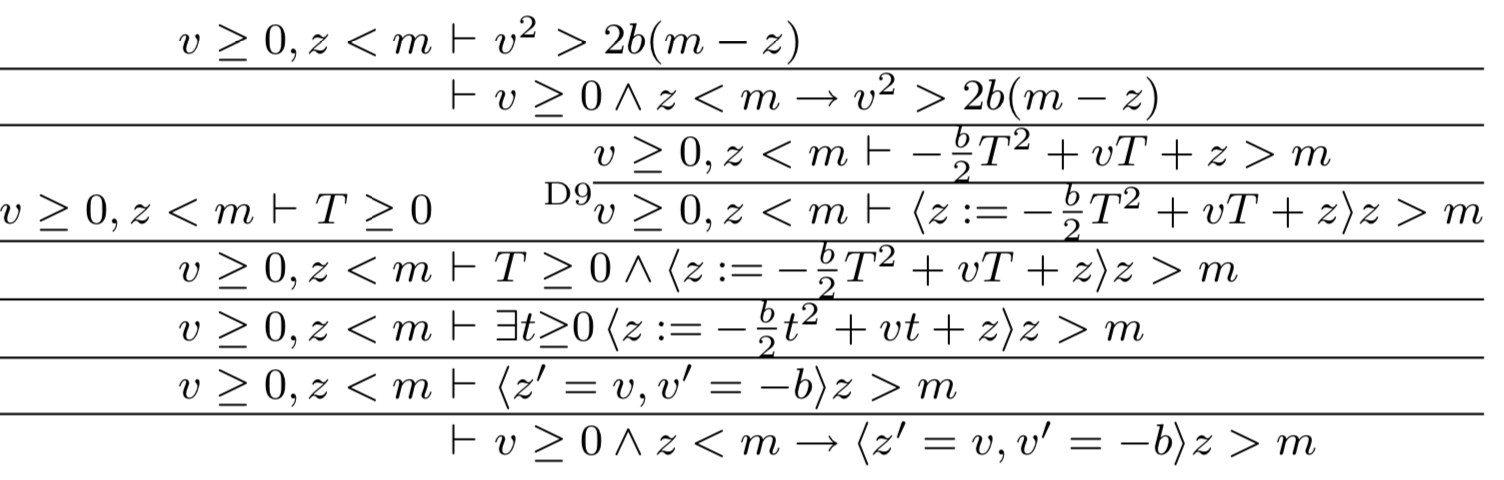
\includegraphics[scale=0.4]{ects-precondition-violation}
   \end{figure}
 \end{block}
\end{frame}

\begin{frame}{Differential Dynamic Logic}{Proof Calculus Application}
  \begin{block}{Deduction modulo for MA violation in braking mode}
    \begin{figure}
      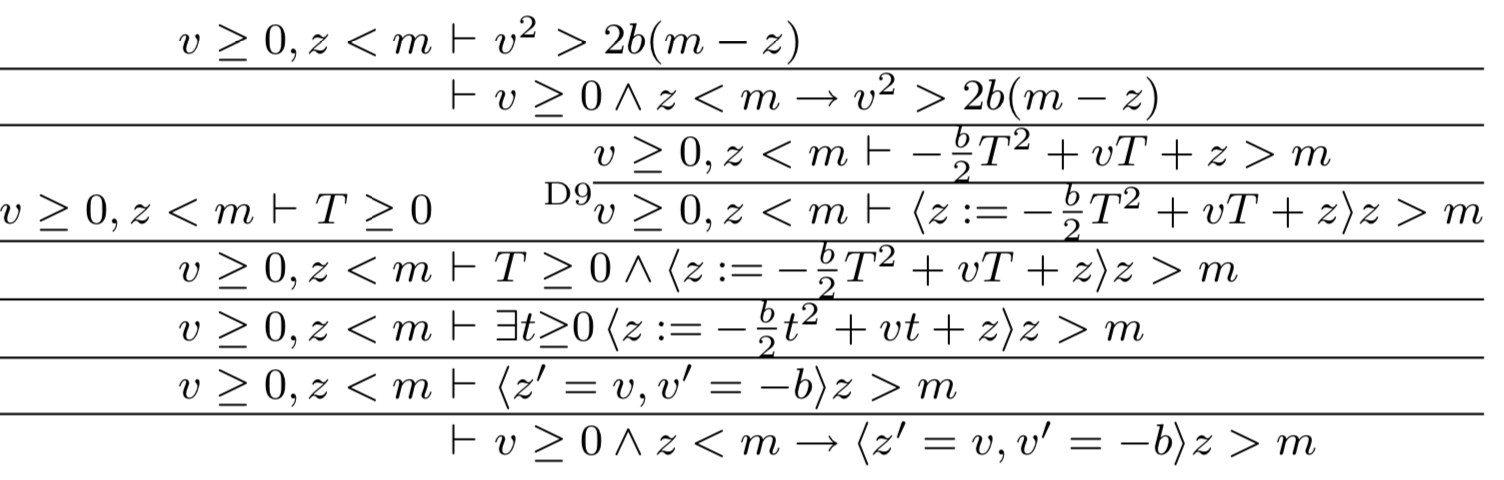
\includegraphics[scale=0.35]{ects-precondition-violation}
    \end{figure}
    \begin{figure}
      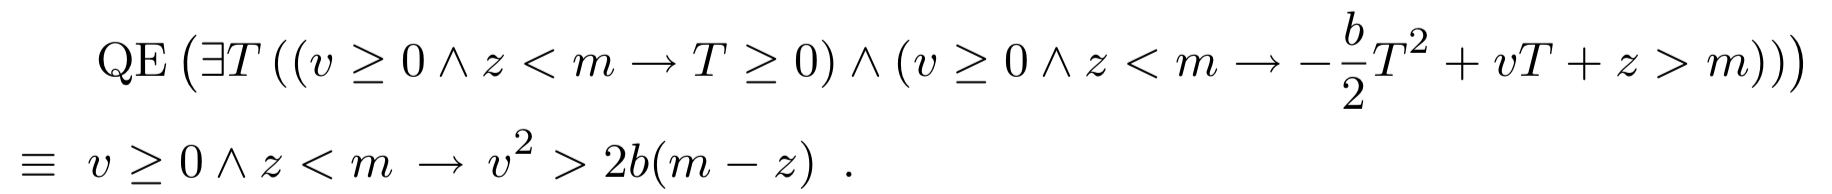
\includegraphics[scale=0.35]{ects-quantifier-elimination}
    \end{figure}
  \end{block}
\end{frame}

\begin{frame}{Differential Dynamic Logic}{Proof Calculus Application}
  \begin{block}{European Train Control System (ETCS) Safety}
    \begin{itemize}
      \item Invariant $\phi \equiv v^2 \leq 2b(m-z) \wedge b > 0 \wedge A \geq
        0$ can be deduced in the manner of finding the violation condition.
      \item The safety proof can then be completed by showing
        \begin{itemize}
          \item Invariant holds initially $\psi \vdash \phi$
          \item $ \phi \to [(ctrl;drive)^*] \phi$ holds.
          \item $\phi \to \varphi_{\textit{post}}$, where
          $\varphi_{\textit{post}} \equiv (\z \leq m)$.
        \end{itemize}
    \end{itemize}
    % \begin{figure}
    %   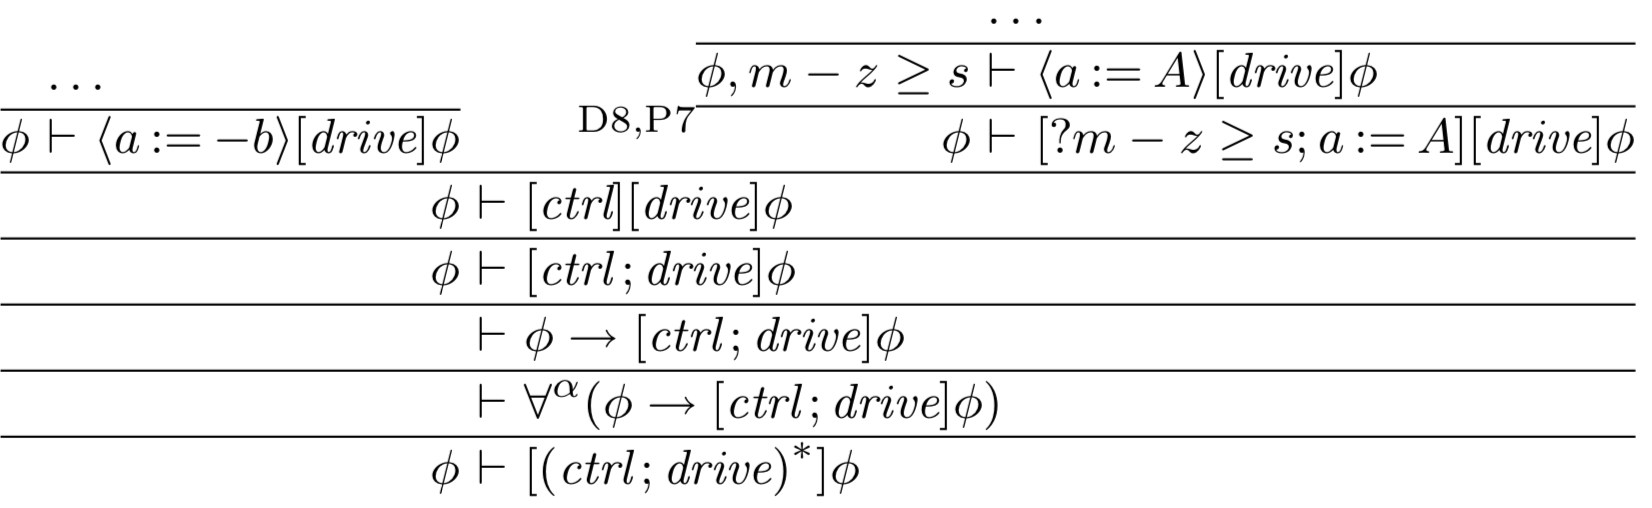
\includegraphics[scale=0.4]{ects-safety-1}
    % \end{figure}
  \end{block}
\end{frame}

\begin{frame}{Differential Dynamic Logic}{Beyond Deductive Verification}
  \begin{itemize}
    \item Verification of a Hybrid System still doesn't guarantee the physical
      system behaves as intended.
    \item Hybrid System involve interaction with real world physics, which can
      never be captured fully by any model.
    \item Runtime monitoring used to obtain real world compliance.
  \end{itemize}
\end{frame}

\begin{frame}{Differential Dynamic Logic}{Beyond Deductive Verification}
  \begin{block}{Runtime Monitoring (ModelPlex)}
  \begin{itemize}
    \item ModelPlex (Mitsch et al.) used $\dL$ for runtime validation of
      systems verified in $\dL$.
    \item Uses $\dL$ to obtain monitoring conditions over Reals (which can be
      checked via SMT solvers)
      \begin{figure}
        \centering
        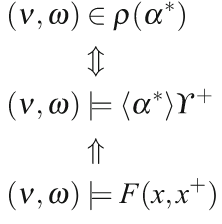
\includegraphics[scale = 0.5]{modelplex}
      \end{figure}
    \item Generate sandbox controller with strong safety guarantees.
  \end{itemize}
\end{block}
\end{frame}

\begin{frame}{Logic and Hybrid System}{Conclusion}
  \begin{itemize}
    \item $\dL$ provides Hybrid Programs - concise notation for Hybrid Systems.
      \pause
    \item A proof calculus suited for verification of CPS and Embedded Systems.
      \pause
    \item Rich toolchain (Keymaera), ModelPlex built on top of $\dL$.
  \end{itemize}
\end{frame}
% \begin{frame}{Differential Dynamic Logic}{Proof Calculus Application}
%   \begin{block}{European Train Control System (ETCS) Safety}
%     \begin{figure}
%       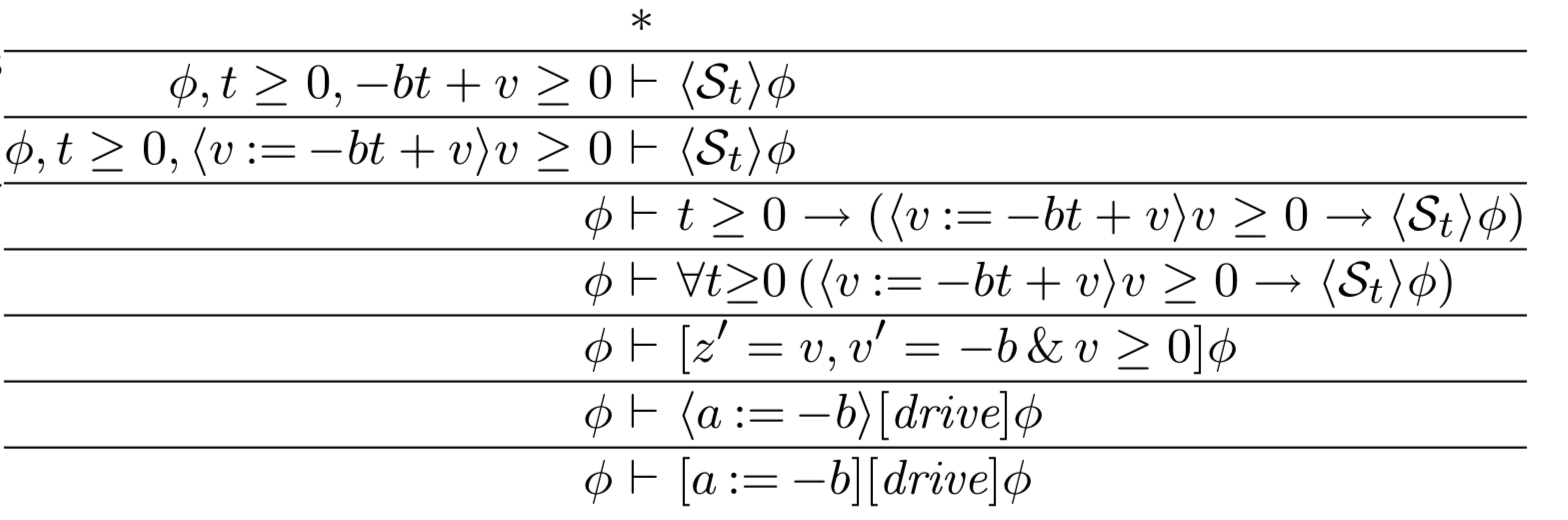
\includegraphics[scale=0.4]{ects-safety-3}
%     \end{figure}
%   \end{block}
% \end{frame}
\end{document}

